%% LaTeX Template for ISIT 2020
%%
%% by Stefan M. Moser, October 2017
%% 
%% derived from bare_conf.tex, V1.4a, 2014/09/17, by Michael Shell
%% for use with IEEEtran.cls version 1.8b or later
%%
%% Support sites for IEEEtran.cls:
%%
%% http://www.michaelshell.org/tex/ieeetran/
%% http://moser-isi.ethz.ch/manuals.html#eqlatex
%% http://www.ctan.org/tex-archive/macros/latex/contrib/IEEEtran/
%%

\documentclass[conference,letterpaper]{IEEEtran}

%% depending on your installation, you may wish to adjust the top margin:
\addtolength{\topmargin}{9mm}

%%%%%%
%% Packages:
%% Some useful packages (and compatibility issues with the IEEE format)
%% are pointed out at the very end of this template source file (they are 
%% taken verbatim out of bare_conf.tex by Michael Shell).
%
% *** Do not adjust lengths that control margins, column widths, etc. ***
% *** Do not use packages that alter fonts (such as pslatex).         ***
%

\usepackage[utf8]{inputenc} 
\usepackage[T1]{fontenc}
\usepackage{url}
\usepackage{ifthen}
\usepackage{cite}
\usepackage[cmex10]{amsmath} % Use the [cmex10] option to ensure complicance
                             % with IEEE Xplore (see bare_conf.tex)

%% Please note that the amsthm package must not be loaded with
%% IEEEtran.cls because IEEEtran provides its own versions of
%% theorems. Also note that IEEEXplore does not accepts submissions
%% with hyperlinks, i.e., hyperref cannot be used.

\interdisplaylinepenalty=2500 % As explained in bare_conf.tex

\usepackage{bm,amsmath,amssymb,multicol,algorithmic,algorithm,enumitem}
\usepackage{times}
\usepackage{dsfont}
\usepackage{xargs}
\newcounter{protocol}
\makeatletter
\newenvironment{protocol}[1][htb]{%
  \let\c@algorithm\c@protocol
  \renewcommand{\ALG@name}{Protocol}% Update algorithm name
  \begin{algorithm}[#1]%
  }{\end{algorithm}
}
\makeatother
\usepackage{mathtools}  
\usepackage{amsmath}
\usepackage{amssymb}
\usepackage{tabulary}
\usepackage{booktabs}
\usepackage{stmaryrd}
\usepackage{color,wrapfig}
\newtheorem{Fact}{Fact}
\newtheorem{Lemma}{Lemma}
\newtheorem{Prop}{Proposition}
\newtheorem{Theorem}{Theorem}
\newtheorem{Def}{Definition}
\newtheorem{Corollary}{Corollary}
\newtheorem{Conjecture}{Conjecture}
\newtheorem{Property}{Property}
\newtheorem{Observation}{Observation}
%\theorembodyfont{\rmfamily}
\newtheorem{Exa}{Example}
\newtheorem{assumption}{A\!\!}
\newtheorem{assumptionA}{G\!\!}
\newtheorem{Remark}{Remark}


\usepackage{shortcuts_OPT}

%%%%%%
% correct bad hyphenation here
\hyphenation{op-tical net-works semi-conduc-tor}

% ------------------------------------------------------------
\begin{document}
\title{Two-Timescale Stochastic EM Algorithms} 

% %%% Single author, or several authors with same affiliation:
% \author{%
%   \IEEEauthorblockN{Stefan M.~Moser}
%   \IEEEauthorblockA{ETH Zürich\\
%                     ISI (D-ITET)\\
%                     CH-8092 Zürich, Switzerland\\
%                     Email: moser@isi.ee.ethz.ch}
% }


%%% Several authors with up to three affiliations:
\author{%
  \IEEEauthorblockN{Belhal Karimi and Ping Li}
  \IEEEauthorblockA{Cognitive Computing Lab\\
  			Baidu Research \\
			10900 NE 8th St. Bellevue, WA 98004\\
                    Email: \{belhal.karimi, ping.li\}@gmail.com}
}


%%% Many authors with many affiliations:
% \author{%
%   \IEEEauthorblockN{Albus Dumbledore\IEEEauthorrefmark{1},
%                     Olympe Maxime\IEEEauthorrefmark{2},
%                     Stefan M.~Moser\IEEEauthorrefmark{3}\IEEEauthorrefmark{4},
%                     and Harry Potter\IEEEauthorrefmark{1}}
%   \IEEEauthorblockA{\IEEEauthorrefmark{1}%
%                     Hogwarts School of Witchcraft and Wizardry,
%                     1714 Hogsmeade, Scotland,
%                     \{dumbledore, potter\}@hogwarts.edu}
%   \IEEEauthorblockA{\IEEEauthorrefmark{2}%
%                     Beauxbatons Academy of Magic,
%                     1290 Pyrénées, France,
%                     maxime@beauxbatons.edu}
%   \IEEEauthorblockA{\IEEEauthorrefmark{3}%
%                     ETH Zürich, ISI (D-ITET), ETH Zentrum, 
%                     CH-8092 Zürich, Switzerland,
%                     moser@isi.ee.ethz.ch}
%   \IEEEauthorblockA{\IEEEauthorrefmark{4}%
%                     National Chiao Tung University (NCTU), 
%                     Hsinchu, Taiwan,
%                     moser@isi.ee.ethz.ch}
% }


\maketitle

%%%%%%
%% Abstract: 
%% If your paper is eligible for the student paper award, please add
%% the comment "THIS PAPER IS ELIGIBLE FOR THE STUDENT PAPER
%% AWARD." as a first line in the abstract. 
%% For the final version of the accepted paper, please do not forget
%% to remove this comment!
%%
\begin{abstract}
The Expectation-Maximization (EM) algorithm is a popular choice for learning latent variable models. 
Variants of the EM have been initially introduced by~\cite{neal1998view}, using incremental updates to scale to large datasets, and by~\cite{wei1990monte, delyon1999}, using Monte Carlo (MC) approximations to bypass the intractable conditional expectation of the latent data for most nonconvex models.
In this paper, we propose a general class of methods called Two-Timescale EM Methods based on a two-stage approach of stochastic updates to tackle an essential nonconvex optimization task for latent variable models.
We motivate the choice of a double dynamic by invoking the variance reduction virtue of each stage of the method on both sources of noise: the index sampling for the incremental update and the MC approximation.
We establish finite-time and global convergence bounds for nonconvex objective functions.
Numerical applications on various models such as deformable template for \emph{image analysis} or nonlinear mixed-effects models for \emph{pharmacokinetics} are also presented to illustrate~our~findings.
\end{abstract}


%% The paper must be self-contained. However, if you are referring to
%% a full version for checking certain proofs, please provide the
%% publically accessible location below.  If the paper is completely
%% self-contained, you can remove the following line from your
%% submission.
\textit{A full version of this paper is accessible at:}
\url{https://hal/} 

\section{Introduction}


Learning latent variable models is critical for modern machine learning problems, see (e.g.,)~\cite{mclachlan2007algorithm} for references.
We formulate the training of such model as an empirical risk minimization problem:
\begin{align} \label{eq:em_motivate}
& \min_{ \param \in \Param }~ \overline{\calL} ( \param ) \eqdef  \calL ( \param ) + \Pen (\param)\\
& \text{with}~~\calL ( \param ) = \frac{1}{n} \sum_{i=1}^n \calL_i( \param) \eqdef  \frac{1}{n} \sum_{i=1}^n \big\{ - \log g( y_i ; \param ) \big\}\eqs,
\end{align}
where $\{y_i\}_{i=1}^n$ are observations, $\Param \subset \rset^d$ is the parameters set and $\Pen : \Param \rightarrow \rset$ is a smooth regularizer.
The objective $ \overline{\calL} ( \param )$ is possibly \emph{nonconvex} and is assumed to be lower bounded. 
In the latent data model, the likelihood $g(y_i ; \param)$, is the marginal of the complete~data likelihood defined as $f(z_i,y_i; \param)$, $g(y_i; \param) = \int_{\Zset} f (z_i,y_i;\param) \mu(\rmd z_i)$, where $\{ z_i \}_{i=1}^n$ are the latent variables.
In this paper, we assume that the complete model belongs to the curved exponential family~\cite{efron1975defining}:
\beq \label{eq:exp}
f(z_i,y_i; \param) = h  (z_i,y_i) \exp \big( \pscal{S(z_i,y_i)}{\phi(\param)} - \psi(\param) \big)\eqs,
\eeq
where $\psi(\param)$, $h(z_i,y_i)$ are scalar functions, $\phi(\param) \in \rset^k$ is a vector function, and $\{S(z_i,y_i) \in \rset^k\}_{i=1}^n$ is the vector of sufficient statistics.
Batch EM~\cite{dempster1977Maximum, wu1983convergence}, the method of reference for \eqref{eq:em_motivate}, is comprised of two steps. 
The \textsf{E-step} computes the conditional expectation of the sufficient statistics of~\eqref{eq:exp}, noted $\overline{\bss}(\param)$: \vspace{-0.1in}

\begin{align}\label{eq:definition-overline-bss}
& \textsf{E-step:}~~\overline{\bss}(\param)= \frac{1}{n} \sum_{i=1}^n \overline{\bss}_i(\param) \\
& \qquad \text{where}  \quad \overline{\bss}_i(\param)= \int_{\Zset} S(z_i,y_i) p(z_i|y_i;\param) \mu(\rmd z_i) \eqsp,
\end{align}
and the \textsf{M-step} is given by
\begin{align}\label{eq:mstep}
\textsf{M-step:}~~\hat{\param} = \overline{\param}( \overline{\bss}(\param) ) \eqdef \argmin_{ \vartheta \in \Param } ~\big\{ \Pen( \vartheta ) + \psi( \vartheta) - \pscal{ \overline{\bss}(\param)}{ \phi ( \vartheta) } \big\} \eqsp.
\end{align}


Two caveats of this method are the following: {\sf(a)} with the explosion of data, the first step of the EM is computationally inefficient as it requires, at each iteration, a full pass over the dataset; and {\sf(b)} the complexity of modern models makes the expectation in \eqref{eq:definition-overline-bss} intractable. 
So far, and to the best of our knowledge, both challenges have been addressed separately, as detailed in the sequel.

\vspace{0.08in}
\noindent \textbf{Prior Work:} Inspired by stochastic optimization procedures,~\cite{neal1998view,cappe2009line} develop respectively an incremental and an online variant of the \textsf{E-step} in models where the expectation is computable, and were then extensively used and studied in~\cite{nguyen2020mini, liang2009online,cappe2011online}.
Some improvements of those methods have been provided and analyzed, globally and in finite-time, in~\cite{karimi2019global} where variance reduction techniques taken from the optimization literature have been efficiently applied to scale the EM algorithm to large datasets.
Regarding the computation of the expectation under the posterior distribution, the Monte Carlo EM (MCEM) has been introduced in~\cite{wei1990monte} where a Monte Carlo (MC) approximation for this expectation is computed. A variant of that algorithm is the Stochastic Approximation of the EM (SAEM) in~\cite{delyon1999} leveraging the power of Robbins-Monro update~\cite{robbins1951stochastic} to ensure pointwise convergence of the vector of estimated parameters using a decreasing stepsize rather than increasing the number of MC samples.
The MCEM and the SAEM have been successfully applied in mixed effects models~\cite{mcculloch1997maximum,hughes1999mixed,baey2016nonlinear} or to do inference for joint modeling of time to event data coming from clinical trials in~\cite{das2010Inferences}, unsupervised clustering in~\cite{ngChoice2003}, variational inference of graphical models in~\cite{BleiVariational2017} among other applications.
An incremental variant of the SAEM was proposed in~\cite{kuhn2019properties} showing positive empirical results but its analysis is limited to asymptotic consideration. 
%Gradient-based methods have been developed and analyzed in~\cite{zhu2017high} but they remain out of the scope of this paper as they tackle the high-dimensionality issue.

\vspace{0.08in}
\noindent \textbf{Contributions:} This paper \textit{introduces} and \textit{analyzes} a new class of methods which purpose is to update two proxies for the target expected quantities in a two-timescale manner. 
Those approximated quantities are then used to optimize the objective function \eqref{eq:em_motivate} for modern examples and settings using the \textsf{M-step} of the EM algorithm.
The main contributions of the paper are:
\begin{itemize}
\item We propose a two-timescale method based on \textsf{(i)} Stochastic Approximation (SA), to alleviate the problem of computing MC approximations, and on \textsf{(ii)} Incremental updates, to scale to large datasets. We describe in details the edges of each level of our method based on variance reduction arguments. Such class of algorithms has two advantages. First, it naturally leverages variance reduction and Robbins-Monro type of updates to tackle large-scale and highly nonlinear learning tasks. Then, it gives a simple formulation as a \textit{scaled-gradient method} which makes the global analysis and the implementation accessible.
\item We also establish global (independent of the initialization) and finite-time (true at each iteration) upper bounds on a classical sub-optimality condition in the nonconvex literature~\cite{jain2017non, ghadimi2013stochastic}, \ie\ the second order moment of the gradient of the objective function. 
We discuss the double dynamic of those bounds due to the two-timescale property of our algorithm update and we theoretically show the advantages of introducing variance reduction in a \emph{Stochastic Approximation}~\cite{robbins1951stochastic} scheme.
\item We stress on the originality of our theoretical findings including such MC sampling noise contrary to existing studies related to the EM where the expectations are computed exactly. 
Adding a layer of MC approximation and the stochastic approximation step to reduce its variance introduce some new technicalities and challenges that need careful considerations and constitues the originality of our paper on the algorithmic and theoretical plans.
\end{itemize}
In Section~\ref{sec:tts} we formalize both incremental and Monte Carlo variants of the EM. Then, we introduce our two-timescale class of EM algorithms for which we derive several global statistical guarantees in Section~\ref{sec:mainanalysis} for possibly \textit{nonconvex} functions.
Section~\ref{sec:numerical} is devoted to numerical illustrations.
The supplementary material of this paper includes proofs of  our theoretical results.


\section{Two-Timescale Stochastic EM Algorithms}\label{sec:tts}


We recall and formalize in this section the different methods found in the literature that aim at solving the intractable expectation and the large-scale problem. 
We then provide the general framework of our method that efficiently tackles the optimization problem \eqref{eq:em_motivate}.


\subsection{Monte Carlo Integration and Stochastic Approximation} 


As mentioned in the Introduction, for complex and possibly nonconvex models, the expectation under the posterior distribution defined in \eqref{eq:definition-overline-bss} is not tractable. In that case, the first solution involves computing a Monte Carlo integration of that latter. 
For all $ i \in \inter$, where $\inter \eqdef \{1, \cdots, n\}$, draw $\{z_{i,m} \sim p(z_i|y_i;\theta)\}_{m=1}^{M}$ samples and compute the MC integration of $\tilde{S}$ of $\overline{\bss}(\param)$ defined by \eqref{eq:definition-overline-bss}:
\beq\label{eq:mcstep}
\textsf{MC-step}:~ \tilde{S} \eqdef \frac{1}{n} \sum_{i=1}^n\frac{1}{M} \sum_{m=1}^M S(z_{i,m}, y_i)\eqs.
\eeq
Then update the parameter via the maximization function $\overline{\param}(\tilde{S} )$.
This algorithm bypasses the intractable expectation issue but is rather computationally expensive in order to reach point wise convergence ($M$ needs to be large).
An alternative to that stochastic algorithm is to use a Robbins-Monro (RM) type of update.
We denote, at iteration $k$, the number of samples $M_k$ and the following MC approximation by $\tilde{S}^{(k+1)}$:
\beq\label{eq:stats}
\begin{split}
& \tilde{S}^{(k+1)} \eqdef \frac{1}{n} \sum_{i=1}^n \tilde{S}^{(k+1)}_i = \frac{1}{n} \sum_{i=1}^n\frac{1}{M_k} \sum_{m=1}^{M_k} S(z_{i,m}^{(k)}, y_i) \\
&  \textrm{where} \quad z_{i,m}^{(k)} \sim p(z_i|y_i;\theta^{(k)})\eqs.
\end{split}
\eeq
Then, the RM update of the sufficient statistics $\hat{\bss}^{(k+1)}$ reads:
\beq\label{eq:rmstep}
\textsf{SA-step}:~ \hat{\bss}^{(k+1)} =  \hat{\bss}^{(k)}  + \gamma_{k+1}(\tilde{S}^{(k+1)} - \hat{\bss}^{(k)} )\eqs,
\eeq
where $\{ \gamma_{k} \}_{k>1} \in (0,1)$ is a sequence of decreasing stepsizes to ensure asymptotic convergence.
The combination of \eqref{eq:stats} and \eqref{eq:rmstep} is called the Stochastic Approximation of the EM (SAEM) and has been shown to converge to a maximum likelihood of the observations under very general conditions~\cite{delyon1999}.
In simple scenarios, the samples $\{z_{i,m}\}_{m=1}^{M}$ are conditionally independent and identically distributed with distribution $p(z_i,\theta)$.
Nevertheless, in most cases, since the loss function between the observed data $y_i$ and the latent variable $z_i$ can be nonconvex, sampling exactly from this distribution is not an option and the MC batch is sampled by Markov Chain Monte Carlo (MCMC) algorithm~\cite{meyn2012markov, brooks2011handbook}.
It has been proved in~\cite{kuhn2004coupling} that \eqref{eq:rmstep} converges almost surely when coupled with an MCMC procedure. 

\noindent \textbf{Role of the stepsize $\gamma_k$:}  The sequence of decreasing positive integers $\{ \gamma_{k} \}_{k>1}$ controls the convergence of the algorithm.
It is inefficient to start with small values for the stepsize $\gamma_k$ and large values for the number of simulations $M_k$. 
Rather, it is recommended that one decreases $\gamma_k$, as in $\gamma_k = 1/k^\alpha$, with $\alpha \in (0,1)$, and keeps a constant and small number $M_k$ bypassing the computationally involved sampling step in \eqref{eq:mcstep}.
 In practice, $\gamma_k$ is set equal to $1$ during the first few iterations to let the iterates explore the parameter space without memory and converge quickly to a neighborhood of the target estimate. 
 The Stochastic Approximation is performed during the remaining iterations ensuring the almost sure convergence of the vector of estimates.

This Robbins-Monro type of update constitutes the \textit{first level} of our algorithm, needed to temper the variance and noise introduced by the Monte Carlo integration.
In the next section, we derive variants of this algorithm to adapt to the sheer size of data of today's applications and formalize the \textit{second level} of our class of two-timescale EM methods.


\subsection{Incremental and Two-Stage Stochastic EM Methods} \label{sec:sEM}

Efficient strategies to scale to large datasets include incremental~\cite{neal1998view} and variance reduced~\cite{chen2018stochastic, johnson:zhang:2013} methods.
We will explicit a general update that covers those latter variants and that represents the \textit{second level} of our algorithm, \ie the incremental update of the noisy statistics $\tilde{S}^{(k+1)}$ in \eqref{eq:stats}. Instead of computing its full batch noted $\tilde{S}^{(k+1)}$ as in \eqref{eq:stats}, the MC approximation is incrementally evaluated through the quantity $\stt^{(k+1)}$ as:
\beq \label{eq:sestep}
\textsf{Inc-step}:~\stt^{(k+1)} = \stt^{(k)} + \rho_{k+1} \big( \StocEstep^{(k+1)}- \stt^{(k)}  \big)\eqs.
\eeq
Note that $\{ \rho_{k} \}_{k>1} \in (0,1)$ is a sequence of stepsizes, $\StocEstep^{(k)}$ is a proxy for $\tilde{S}^{(k)}$ defined in \eqref{eq:stats}.
If the stepsize is equal to $1$ and $\StocEstep^{(k)} = \tilde{S}^{(k)}$, i.e., computed in a full batch manner as in \eqref{eq:stats}, then we recover the SAEM algorithm.
Also if $\rho_{k}=1$, $\gamma_{k}=1$ and $\StocEstep^{(k)} = \tilde{S}^{(k)}$, then we recover the MCEM.

\vspace{0.08in}
\noindent \textbf{Remarks on Table~\ref{alg:prox}:} For all methods, we define a random index drawn at iteration $k$, noted $i_k \in \inter$, and $\tau_i^k = \max \{ k' : i_{k'} = i,~k' < k \}$ as the iteration index where $i \in \inter$ is last drawn prior to iteration $k$.

 \begin{protocol}[H]
  \floatname{algorithm}{Table}
\caption{Proxies for the Incremental-step~\eqref{eq:sestep}}\label{alg:prox}
  \begin{algorithmic}[1]
  \STATE \textsf{\ISAEM\ }$\hspace{0.7cm} \StocEstep^{(k+1)} = \StocEstep^{(k)} + n^{-1} \big( \tilde{S}_{i_k}^{(k)}  - \tilde{S}_{i_k}^{(\tau_{i_k}^k)} \big) \label{eq:isaem}$
    \STATE \textsf{\SAEMVR\ }$\hspace{0.5cm} \StocEstep^{(k+1)}  = \stt^{(\ell(k))} +  \big( \tilde{S}_{i_k}^{(k)}  -\tilde{S}_{i_k}^{(\ell(k))}   \big) \label{eq:vrsaem}$
      \STATE \textsf{\FISAEM\ }$\hspace{0.6cm} \StocEstep^{(k+1)} = \overline{\StocEstep}^{(k)} + \big( \tilde{S}_{i_k}^{(k)}  - \tilde{S}_{i_k}^{(t_{i_k}^k)} \big) \label{eq:fisaem}$\\
             $ \hspace{1.95cm} \overline{\StocEstep}^{(k+1)} = \overline{\StocEstep}^{(k)} + n^{-1} \big( \tilde{S}_{j_k}^{(k)}  - \tilde{S}_{j_k}^{(t_{j_k}^k)} \big)$
  \end{algorithmic}
\end{protocol}

The proposed \FISAEM\ method draws \emph{two} indices \emph{independently} and uniformly as $i_k, j_k \in \inter$. 
Thus, we define $t_j^k = \{ k' : j_{k'} = j , k' < k \}$ to be the iteration index where the sample $j \in \inter$ is last drawn as $j_k$ prior to iteration $k$ in addition to $\tau_i^k$ which was defined \wrt $i_k$.


Recall $\tilde{S}_{i_k}^{(k)}=  \frac{1}{M_k} \sum_{m=1}^{M_k} S(z_{i_k,m}^{(k)}, y_{i_k})$ where $z_{i_k,m}^{(k)}$ are samples drawn from $ p(z_{i_k}|y_{i_k};\theta^{(k)})$.
The stepsize in~\eqref{eq:sestep} is set to $\rho_{k+1} = 1$ for the \ISAEM\ method and we initialize with $\StocEstep^{(0)} = \tilde{S}^{(0)}$; $\rho_{k+1} = \rho$ is  constant for the \SAEMVR\ and \FISAEM\ methods. Note that we initialize as follows $\overline{\StocEstep}^{(0)} = \tilde{S}^{(0)}$ for the \FISAEM\ which can be seen as a slightly modified version of SAGA inspired by~\cite{reddi2016fast}.
For \SAEMVR\, we set an epoch size of $m$ and we define $\ell(k) \eqdef m \lfloor k/m \rfloor$ as the first iteration number in the epoch that iteration $k$ is in.


\vspace{0.08in}
\noindent \textbf{Two-Timescale Stochastic EM methods:}
We now introduce the general method derived using the two variance reduction techniques described above.
Algorithm~\ref{alg:ttsem} leverages both levels \eqref{eq:rmstep} and \eqref{eq:sestep} in order to output a vector of fitted parameters $\hat{\param}^{({\sf K}_{\sf m })}$ where ${\sf K}_{\sf m }$ is the total number of iterations.
\begin{algorithm}[H]
\caption{Two-Timescale Stochastic EM methods.}\label{alg:ttsem}
  \begin{algorithmic}[1]
  \STATE \textbf{Input:} $\hat{\param}^{(0)} \leftarrow 0$, $\hat{\bss}^{(0)} \leftarrow \tilde{S}^{(0)}$, $\{\gamma_k\}_{k>0}$, $\{\rho_k\}_{k>0}$ and $ {\sf K}_{\sf m }\in \mathbb{N}^*$.
%  \STATE Set the terminating iteration number, $K \in \{0,\dots,{\sf K}_{\sf m }-1\}$, as a discrete r.v.~with:\vspace{-.1cm}
%  \beq \label{eq:random}
%   P( K = k ) = \frac{ \gamma_{k} }{\sum_{\ell=0}^{{\sf K}_{\sf m }-1} \gamma_\ell} = \frac{\gamma_k}{{\sf P}_{\sf m}}\eqs.\vspace{-.2cm} 
%  \eeq
  \FOR {$k=0,1,2,\dots, {\sf K}_{\sf m } - 1$}
  \STATE Draw index $i_k \in \inter$ uniformly (and $j_k \in \inter$ for \FISAEM).
     \STATE Compute $\tilde{S}_{i_k}^{(k)}$ using the {\sf MC-step} \eqref{eq:mcstep},  for the drawn indices.
   \STATE Compute the surrogate sufficient statistics $\StocEstep^{(k+1)}$ using Lines~\ref{eq:isaem}, \ref{eq:vrsaem} or \ref{eq:fisaem} in Table~\ref{alg:prox}.
   \STATE Compute $\stt^{(k+1)}$ and $\hat{\bss}^{(k+1)}$ using respectively \eqref{eq:sestep} and \eqref{eq:rmstep}:
\beq \label{eq:twolevels}
\begin{split}
& \stt^{(k+1)} = \stt^{(k)} + \rho_{k+1} \big( \StocEstep^{(k+1)}- \stt^{(k)}  \big)\\
&  \hat{\bss}^{(k+1)} =  \hat{\bss}^{(k)}  + \gamma_{k+1}(\stt^{(k+1)} - \hat{\bss}^{(k)} )
\end{split}
\eeq
   \STATE Update $\hat{\param}^{(k+1)} = \overline{\param}(  \hat{\bss}^{(k+1)}) $ via the {\sf M-step}.
\ENDFOR
  \end{algorithmic}
\end{algorithm}
The update in \eqref{eq:twolevels} is said to have a two-timescale property as the stepsizes satisfy $\lim_{k \to \infty} \gamma_k/\rho_k < 1$ such that $ \tilde{S}^{(k+1)} $  is updated at a faster time-scale, determined by $\rho_{k+1}$, than $\hat{\bss}^{(k+1)}$, determined by $\gamma_{k+1}$.
The next section introduces the main results of this paper and establishes global and finite-time bounds for the three different updates of our scheme. 

%We first recall the main notations introduced in the previous section:\vspace{-0.1in}
%
%\begin{table}[htbp]
%%\caption{Table of Notations}
%\begin{center}% used the environment to augment the vertical space
%% between the caption and the table
%\begin{tabular}{r c p{10cm} }
%\toprule
%$\tilde{S}$ & $\triangleq$ &  MC approximation of its expected counterpart $\overline{\bss}$ at index $i \in \inter$\\
%$\StocEstep$ & $\triangleq$ & proxy of the MC approximation $\tilde{S}$ and updated incrementally according to Table~\ref{alg:prox}\\  
%$\stt$ & $\triangleq$ & variance-reduced quantity in~\eqref{eq:sestep} and related to stepsize $\rho$\\
%$\hat{\bss}$ & $\triangleq$ & statistics resulting from the Robbins-Monro procedure in~\eqref{eq:rmstep} and related to stepsize $\gamma$\\
%\bottomrule
%\end{tabular}
%\end{center}
%\label{tab:notations}
%\end{table}


\section{Finite Time Analysis of the Two-Timescale Scheme} \label{sec:mainanalysis}
Following~\cite{cappe2009line}, it can be shown that stationary points of the objective function \eqref{eq:em_motivate} corresponds to the stationary points of the following \textit{nonconvex} Lyapunov function:
\beq\label{eq:em_sspace}
\min_{ {\bss} \in \Sset }~  V ( {\bss} ) \eqdef \overline\calL( \op(\bss) ) =  \frac{1}{n} \sum_{i=1}^n {\cal L}_i (  \op(\bss) )+ \Pen (  \op(\bss) ) \eqs,
\eeq
that we propose to study in this article.


\subsection{Assumptions and Intermediate Lemmas}




Several important assumptions required to derive convergence guarantees read as follows:
\begin{assumption}\label{ass:compact}
The sets $\Zset, \Sset$ are compact. There exist constants $C_{\Sset}, C_{\Zset}$ such that:
\beq \textstyle \label{eq:compact}
C_{\Sset} \eqdef \max_{ \bss, \bss' \in \Sset } \| \bss - \bss' \| < \infty,~~~~C_{\Zset} \eqdef \max_{i \in \inter} \int_{\Zset} | S(z,y_i) | \mu( \rmd z ) < \infty.
\eeq
\end{assumption}

\begin{assumption}\label{ass:expected}
For any $i \in \inter$, $z \in \Zset$, $\param, \param' \in {\rm int} (\Param)^2$, we have $\big| p( z | y_i; \param ) - p( z | y_i; \param' ) \big| \leq  \Lip{p} \| \param - \param' \|$ where ${\rm int} (\Param)$ denotes the interior of $\Param$.
\end{assumption}
We also recall that we consider curved exponential family models assuming the following:
\begin{assumption} \label{ass:reg}
For any $\bm{s} \in \Sset$, the function $\param \mapsto L(s,\param) \eqdef \Pen( \param ) + \psi( \param) - \pscal{ \bss}{ \phi ( \param) }$ admits a unique global minimum $\mstep{\bss} \in {\rm int}(\Param)$.

In addition, $\jacob{\phi}{\param}{\overline{\param}(\bss )}$, the Jacobian of the function $\phi$ at $\param$, is full rank, $\Lip{p}$-Lipschitz and $\overline{\param}( \bss )$ is $\Lip{t}$-Lipschitz.
\end{assumption}
We denote by $\hess{L}{\param}(\bss,\param)$ the Hessian (w.r.t to $\param$ for a given value of $\bss$) of the function $\param \mapsto L(\bss,\param)= \Pen(\param) + \psi(\param) -\pscal{\bss}{\phi(\param)}$, and define $\operatorname{B}( \bss ) \eqdef\jacob{ \phi }{ \param }{ \mstep{\bss} } \Big( \hess{L}{\param}( {\bss},  \mstep{\bss} )  \Big)^{-1} \jacob{ \phi }{ \param }{ \mstep{\bss} }^\top$.
\begin{assumption}\label{ass:eigen}
It holds that $ \upsilon_{\max} \eqdef \sup_{\bss \in \Sset} \| \operatorname{B}( \bss ) \| < \infty$ and $0 < \upsilon_{\min}  \eqdef \inf_{\bss \in \Sset} \lambda_{\rm min} ( \operatorname{B}( \bss ) )$.
There exists a constant $\Lip{b}$ such that for all $\bss, \bss' \in \Sset^2$, we have $ \| \operatorname{B}( \bss ) - \operatorname{B}( \bss' )  \| \leq \Lip{b} \| {\bss} - {\bss}' \|$.
\end{assumption}
The class of algorithms we develop in this paper is composed of two levels where the second stage corresponds to the variance reduction trick used in~\cite{karimi2019global} in order to accelerate incremental methods and reduce the variance introduced by the index sampling. 
The first stage is the Robbins-Monro update that aims at reducing the Monte Carlo noise of $\tilde{S}^{(k+1)}$ at iteration $k$:
\beq\label{eq:mcerror}
\eta_{i}^{(k)} \eqdef \tilde{S}_{i}^{(k)} -  \overline{\bss}_i(\vartheta^{(k)})\quad  \textrm{for all} \quad  i \in \inter \quad \textrm{and} \quad  k > 0 \eqs.
\eeq
For instance, we consider that the MC approximation is unbiased if for all $ i \in \inter$ and $m \in [M]$, the samples $z_{i,m} \sim p(z_i|y_i;\theta)$ are i.i.d. under the posterior distribution, \ie $\EE[\eta_{i}^{(k)}|{\cal F}_k] = 0$ where  ${\cal F}_k$ is the filtration up to iteration $k$.
The following results are derived under the assumption that the fluctuations implied by the approximation are bounded:
%\begin{assumption}\label{ass:mcerror}
%There exist a positive sequence of MC batch size $\{M_r\}_{r > 0}$ and constants $(c, c_{\eta})$ such that for all $k >0$, $i \in \inter$ and $\vartheta \in \Theta$:
%\beq\label{eq:boundederror}
%\EE [\| \eta_{i}^{(r)}\|^2 ] \leq \frac{c_{\eta}}{M_r} \quad \textrm{and} \quad \EE[\| \EE[\eta_{i}^{(r)}|{\cal F}_r]\|^2] \leq \frac{c}{M_r}\eqs.
%\eeq
%\end{assumption}\vspace{-0.1in}
\begin{assumption}\label{ass:mcerror}
For all $k >0$, $i \in \inter$, it holds: 
$\EE [\| \eta_{i}^{(k)}\|^2 ] < \infty \quad \textrm{and} \quad \EE[\| \EE[\eta_{i}^{(k)}|{\cal F}_k]\|^2] < \infty \eqs.$
\end{assumption}
Note that typically, the controls exhibited above are vanishing when the number of MC samples $M_k$ increases~with~$k$.
We now state two important results on the Lyapunov function; its smoothness:
\begin{Lemma} \label{lem:smooth}
\cite{karimi2019global} Assume A\ref{ass:compact}-A\ref{ass:eigen}.  
For all $\bss,\bss' \in \Sset$ and $i \in \inter$, we have
\beq \label{eq:smooth}
\| \overline{\bss}_i ( \overline{\param} ({\bss})) - \overline{\bss}_i ( \overline{\param} ({\bss}' )) \| \leq \Lip{{\bss}} \| {\bss} - {\bss}' \|,~~\| \grd  V ( {\bss} ) - \grd  V ( {\bss}' ) \| \leq \Lip{V} \| {\bss} - {\bss}' \|\eqs,
\eeq
where $\Lip{\bss} \eqdef C_{\Zset} \Lip{p} \Lip{t}$ and $\Lip{V}  \eqdef \upsilon_{\max} \big( 1 + \Lip{{\bss}} \big) + \Lip{b} C_{\Sset}$.
\end{Lemma}
We also establish a growth condition on the gradient of $V$ related to the mean field of the algorithm:
\begin{Lemma}\label{lem:growth}
Assume A\ref{ass:reg} and A\ref{ass:eigen}. For all $\bss \in \Sset$,
\beq \label{eq:semigrad}
\upsilon_{\min}^{-1} \pscal{\grd V ( {\bss} ) }{ {\bss} - \os( \op ({\bss})) } \geq \| {\bss} - \os( \op ({\bss})) \|^2 \geq \upsilon_{\max}^{-2} \| \grd V ( {\bss} ) \|^2\eqs.
\eeq
\end{Lemma}

We present in the following sections a finite-time and global (independent of the initialization) analysis of both the incremental and two-timescale variants our method. 


\subsection{Global Convergence of Incremental Stochastic EM Algorithms}


The following result for the \ISAEM\ algorithm is derived under the control of the Monte Carlo fluctuations as described by Assumption A\ref{ass:mcerror} and is built upon an intermediary Lemma, characterizing the quantity of interest $( \stt^{(k+1)} - \hat{\bss}^{(k)} )$:
\begin{Lemma}\label{lem:meanfield_isaem}
 Assume A\ref{ass:compact}. The \ISAEM\ update~\eqref{eq:isaem} is equivalent to the following update on the statistics $\hat{\bss}^{(k+1)} =  \hat{\bss}^{(k)}  + \gamma_{k+1} \big(  \sum_{i=1}^n \tilde{S}_i^{(\tau_i^k)} - \hat{\bss}^{(k)} \big)$.
Also:
\beq\notag
\EE[\stt^{(k+1)} - \hat{\bss}^{(k)}] = \EE[\overline{\bss}^{(k)} - \hat{\bss}^{(k)}] + \left(1 - \frac{1}{n} \right) \EE\left[\frac{1}{n} \sum_{i=1}^n \tilde{S}_i^{(\tau_i^k)}- \overline{\bss}^{(k)}\right]  +\frac{1}{n}\EE[\eta_{i_k}^{(k+1)}]\eqsp,
\eeq
where $\overline{\bss}^{(k)}$ is defined by \eqref{eq:definition-overline-bss} and $\tau_i^k = \max \{ k' : i_{k'} = i,~k' < k \}$.
\end{Lemma}
Then, the following non-asymptotic convergence rate can be derived for the \ISAEM\ algorithm:
\begin{Theorem}\label{thm:isaem}
Assume A\ref{ass:compact}-A\ref{ass:mcerror}.
Consider the \ISAEM\ sequence $\{\hat{\bss}^{(k)}\}_{k>0} \in \mathcal{S}$ obtained with $\rho_{k+1}=1$ for any $k \leq {\sf K}_{\sf m }$ where ${\sf K}_{\sf m }$ is a positive integer. 
Let $\{\gamma_{k} = 1/(k^a \alpha c_1 \overline{L})\}_{k>0}$, where $a \in (0,1)$, be a sequence of stepsizes, $c_1 = \upsilon_{\min}^{-1}$, $\alpha = \max\{8, 1+6\upsilon_{\min}\}$, $\overline{L} = \max\{ \Lip{\bss} , \Lip{V} \}$, $\beta = c_1 \overline{L}/n$. Then:
\beq\notag
\upsilon_{\max}^{-2}\sum_{k=0}^{{\sf K}_{\sf m }} \tilde{\alpha}_k \EE [\|\grd V( \hs{k} )\|^2]  \leq   \EE  [V( \hs{0} ) - V( \hs{{\sf K}_{\sf m }} ) ] + \sum_{k=0}^{{\sf K}_{\sf m }-1} \tilde{\Gamma}_k         \EE [\| \eta_{i_k}^{(k)}\|^2] \eqs.
\eeq
\end{Theorem} 
Note that, in Theorem~\ref{thm:isaem}, the convergence bound is composed of an initialization term $V( \hs{0} ) - V( \hs{{\sf K}_{\sf m }} )$ and suffers from the Monte Carlo noise introduced by the posterior sampling step, see the second term on the RHS of the inequality. 
We observe, in the next section, that when variance reduction is applied ($\rho_k < 1$), a second phase of convergence will be included in our bounds.


\subsection{Global Convergence of Two-Timescale Stochastic EM Algorithms}


We now deal with the analysis of Algorithm~\ref{alg:ttsem} when variance reduction is applied \ie\ $\rho <1$.
Two important intermediate Lemmas are needed in order to establish finite-time bounds for the \SAEMVR\ and the \FISAEM\ methods.
We first derive an identity for the drift term of the \SAEMVR\ :
\begin{Lemma}\label{lem:auxvrsaem}
Consider the \SAEMVR\ update~\eqref{eq:vrsaem} with $\rho_k = \rho$, it holds for all $k>0$ 
\beq\notag
\begin{split}
  \EE [\| \hs{k} - \stt^{(k+1)}\|^2 ] \leq& 2\rho^2 \EE[ \| \hs{k} - \os^{(k)} \|^2] +  2\rho^2\Lip{\bss}^2 \EE[ \| \hs{k} - \hs{\ell(k)} \|^2 ]\\
  &+2(1-\rho)^2 \EE[ \| \hs{(k)} - \stt^{(k)} \|^2 ]+ 2\rho^2\EE[\|\eta_{i_k}^{(k+1)} \|^2]\eqs,
\end{split}
\eeq
where we recall that $\ell(k)$ is the first iteration number in the epoch that iteration $k$ is in.
\end{Lemma}
The second one derives an identity for the quantity $\EE[ \| \hs{k} - \stt^{(k+1)}   \|^2 ]$ using the \FISAEM\ update:
\begin{Lemma}\label{lem:aux1}
Consider the \FISAEM\ update~\eqref{eq:fisaem} with $\rho_k = \rho$. It holds for all $k>0$ that
\beq\notag
\begin{split}
  \EE [\| \hs{k} - \stt^{(k+1)}\|^2 ] \leq& 2\rho^2 \EE[ \| \hs{k} - \os^{(k)} \|^2] +  2\rho^2\frac{\Lip{\bss}^2}{n}
\sum_{i=1}^n \EE[ \| \hs{k} - \hs{t_i^k} \|^2 ]\\
  &+2(1-\rho)^2 \EE[ \| \hs{(k)} - \stt^{(k)} \|^2 ]+ 2\rho^2\EE[\|\eta_{i_k}^{(k+1)} \|^2]\eqsp,
\end{split}
\eeq
where $\Lip{\bss}$ is the smoothness constant defined in Lemma~\ref{lem:smooth}.
\end{Lemma}
Let $K$ be an independent discrete r.v.~drawn from $\{1,\dots,{\sf K}_{\sf m }\}$ with distribution  $\{ \gamma_{k+1}/ {\sf P}_{\sf m}\}_{k=0}^{{\sf K}_{\sf m } - 1 }$, then, for any ${\sf K}_{\sf m } >0 $, the convergence criterion used in our study reads
\beq\notag
\EE[ \| \grd V( \hs{K} ) \|^2 ]  = \frac{1}{{\sf P}_{\sf m}} \sum_{k=0}^{{\sf K}_{\sf m }-1} \gamma_{k+1} \EE[ \| \grd V( \hs{k} ) \|^2 ] \eqs,
\eeq 
where ${\sf P}_{\sf m} = \sum_{\ell=0}^{{\sf K}_{\sf m }-1} \gamma_\ell$ and the expectation is over the stochasticity of the algorithm.
Denote $\Delta V = V( \hs{0} ) - V( \hs{{\sf K}_{\sf m }})$. We now state the main result regarding the \SAEMVR\ method:
\begin{Theorem}\label{thm:vrsaem}
Assume A\ref{ass:compact}-A\ref{ass:mcerror}.
Consider the \SAEMVR\ sequence $\{\hat{\bss}^{(k)}\}_{k>0} \in \mathcal{S}$ for any $k \leq {\sf K}_{\sf m }$ where ${\sf K}_{\sf m }$ is a positive integer. 
Let $\{\gamma_{k+1} = 1/(k^a \overline{L})\}_{k>0}$, where $a \in (0,1)$, be a sequence of stepsizes, $\overline{L} = \max \{\Lip{\bss}, \Lip{V} \}$, $\rho = \mu/( c_1 \overline{L}  n^{2/3})$, $m = n c_1^2/(2 \mu^2+\mu c_1^2)$ and a constant $\mu \in (0,1)$. Then:
\beq\notag
\EE[ \| \grd V( \hs{K} ) \|^2 ] \leq  \frac{2 n^{2/3} \overline{L}}{\mu {\sf P}_{\sf m} \upsilon_{\min}^2\upsilon_{\max}^2}\left( \EE[ \Delta V ]+  \sum_{k=0}^{{\sf K}_{\sf m }-1}  \tilde{\eta}^{(k+1)}\hspace{-0.1cm} + \chi^{(k+1)} \EE[\| \hs{k} - \stt^{(k)}\|^2]\right)  \eqsp.
\eeq
\end{Theorem}
Furthermore, the \FISAEM\ method has the following convergence rate:
\begin{Theorem}\label{thm:fisaem}
Assume A\ref{ass:compact}-A\ref{ass:mcerror}.
Consider the \FISAEM\ sequence $\{\hat{\bss}^{(k)}\}_{k>0} \in \mathcal{S}$ for any $k \leq {\sf K}_{\sf m }$ where ${\sf K}_{\sf m }$ be a positive integer.
Let $\{\gamma_{k+1} = 1/(k^a \alpha c_1 \overline{L}) \}_{k>0}$, where $a \in (0,1)$, be a sequence of positive stepsizes, $\alpha =\max\{2, 1+2\upsilon_{\min}\}$, $\overline{L} = \max\{ \Lip{\bss} , \Lip{V} \}$, $\beta = 1/(\alpha n)$, $\rho = 1/(\alpha c_1 \overline{L}n^{2/3})$ and $c_1(k\alpha-1) \geq c_1(\alpha-1) \geq 2$, $\alpha \geq 2$. Then:
\beq\notag
 \EE[ \| \grd V( \hs{K} ) \|^2 ] \leq \frac{4\alpha  \overline{L} n^{2/3}}{{\sf P}_{\sf m}\upsilon_{\min}^2\upsilon_{\max}^2} \left( \EE \big[ \Delta V \big]   + \sum_{k=0}^{{\sf K}_{\sf m }-1}  \Xi^{(k+1)}  +\Gamma^{(k+1)} \EE [\| \hs{k} - \stt^{(k)}\|^2 ]\right)\eqs.
\eeq
\end{Theorem}
Note that in those two bounds, the quantities $\tilde{\eta}^{(k+1)} $ and $ \Xi^{(k+1)} $ depend only on the Monte Carlo noises $\EE [\| \eta_{i_k}^{(k)}\|^2 ]$, $\EE[\| \EE[\eta_{i}^{(r)}|{\cal F}_r]\|^2]$, bounded under Assumption A\ref{ass:mcerror}, and some constants.

\vspace{0.08in}
\noindent \textit{Remarks:} Theorem~\ref{thm:vrsaem} and Theorem~\ref{thm:fisaem} exhibit in their convergence bounds \emph{two different phases}. 
The upper bounds display a \emph{bias term} due to the initial conditions, \ie the term $ \Delta V$, and a \emph{double dynamic} burden exemplified by the term $\EE [\| \hs{k} -  \tilde{S}^{(k)} \|^2] $. 
Indeed, the following remarks are worth doing on this quantity: \textsf{(i)} This term is the price we pay for the two-timescale dynamic and corresponds to the gap between the two \emph{asynchronous} updates (one on  $\hs{k}$ and the other on $ \tilde{S}^{(k)}$).  
\textsf{(ii)} It is readily understood that if $\rho = 1$, \ie\ there is no variance reduction, then for any $k >0$
\beq\notag
\EE [\| \hs{k}  - \stt^{(k)}   \|^2] = \EE [\| \StocEstep^{(k+1)} - \stt^{(k+1)} \|^2]= 0 \quad \textrm{with} \quad \hs{0} = \tilde{S}^{(0)}=0 \eqsp,
\eeq
which strengthen the fact that this quantity characterizes the impact of the variance reduction technique introduced in our class of methods. 
The following Lemma characterizes this gap:
\begin{Lemma} \label{lem:gap_dynamics}
Considering a decreasing stepsize $\gamma_k \in (0,1)$ and a constant $\rho \in (0,1)$, we have
\beq\notag
\begin{split}
\EE [\| \hs{k} - \stt^{(k)}   \|^2]  \leq \frac{\rho}{1-\rho}\sum_{\ell = 0}^k (1-\gamma_{\ell} )^2 (   \StocEstep^{(\ell)} - \stt^{(\ell)})\eqs,
\end{split}
\eeq
where $\StocEstep^{(\ell)}  $ is defined either by Line~\ref{eq:vrsaem} (\SAEMVR\ ) or Line~\ref{eq:fisaem} (\FISAEM\ ).
\end{Lemma}



%\section{Numerical Examples}\label{sec:numerical}
%
%
%\begin{wrapfigure}[11]{r}{2.8in}\vspace{-0.5in}
%\begin{center}
%%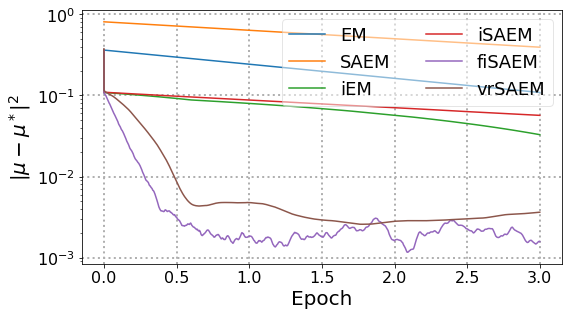
\includegraphics[width=2.5in]{pic_paper/tts_gmm_n100k.png}
%\includegraphics[width=2.5in]{fig/figgmm.eps}
%\end{center}
%\vspace{-0.1in}
%\caption{Precision $|\mu^{(k)} - \mu^*|^2$ per epoch\vspace{0.2in}}
%\label{fig:gmm_tts}%\vspace{0.3in}
%\end{wrapfigure}
%
%This section presents several numerical applications for our proposed class of Algorithms~\ref{alg:ttsem}.
%
%
%\subsection{Gaussian Mixture Models}
%
%
%We begin by a simple and illustrative example.
%The authors acknowledge that the following model can be trained using deterministic EM-type of algorithms but propose to apply stochastic methods, including theirs, in order to compare their performances.
%Given $n$ observations $\{y_i\}_{i=1}^n$, we want to fit a Gaussian Mixture Model (GMM) whose distribution is modeled as a mixture of $M$ Gaussian components, each with a unit variance. 
%Let $z_i \in \inter[M]$ be the latent labels of each component, the complete log-likelihood is defined as follows:
%\beq \notag \textstyle
% \log f( z_i, y_i; \param) =
%\sum_{m=1}^{M} \indiacc{m}(z_i) \left[ \log(\omega_m) - \mu_m^2/2 \right] + \sum_{m=1}^M \indiacc{m}(z_i) \mu_m y_i + {\rm constant} \eqsp.
%\eeq
%where $\param \eqdef (\bomega, \bmu)$ with $\bomega= \{\omega_{m}\}_{m=1}^{M-1}$ are the mixing weights with the convention $\omega_M= 1 - \sum_{m=1}^{M-1} \omega_m$  and $\bmu= \{\mu_m \}_{m =1}^M$ are the means.  
%We use the penalization $\Pen(\param)= \frac{\delta}{2}\sum_{m=1}^M \mu_m^2 - \log \Dir(\bomega; M, \epsilon)$ where $\delta > 0$ and $\Dir(\cdot; M,\epsilon)$ is the $M$ dimensional symmetric Dirichlet distribution with concentration parameter $\epsilon > 0$.
%The constraint set is given by $\Param = \{ \omega_m,~m=1,...,M-1 : \omega_m \geq 0,~\sum_{m=1}^{M-1} \omega_m \leq 1\} \times \{ \mu_m \in \rset ,~m=1,...,M \}$. 
%In the following experiments on synthetic data, we generate $50$ synthetic datasets of size $n = 10^5$ from a GMM model with $M=2$ components of means $\mu_1 = - \mu_2 = 0.5$.
%We run the EM method until convergence (to double precision) to obtain the ML estimate $\mu^\star$ averaged on $50$ datasets. 
%We compare the EM, iEM (incremental EM), SAEM, \ISAEM, \SAEMVR\ and \FISAEM\ methods in terms of their precision measured by $| \mu - \mu^\star |^2$. 
%We set the stepsize of the \textsf{SA-step} for all method as $\gamma_k = 1/k^{\alpha}$ with $\alpha = 0.5$, and the stepsize $\rho_k$ for the \SAEMVR\ and the \FISAEM\ to a constant stepsize equal to $1/n^{2/3}$. 
%The number of MC samples is fixed to $M=10$.
%Figure~\ref{fig:gmm_tts} shows the precision $|\mu - \mu^*|^2$ for the different methods through the epoch(s) (one epoch equals $n$ iterations). 
%The \SAEMVR\ and \FISAEM\ methods outperform the other stochastic methods, supporting the benefits of our scheme.
%
%
%\subsection{Deformable Template Model for Image Analysis}
%
%
%Let $(y_i, i \in \inter)$ be observed gray level images defined on a grid of pixels.
%Let $u \in \mathcal{U} \subset \rset^2$ denote the pixel index on the image and $x_u \in \mathcal{D} \subset \rset^2$ its location.
%The model used in this experiment suggests that each image $y_i$ is a deformation of a template, noted $I: \mathcal{D} \to \rset$, common to all images of the dataset:
%\beq\label{eq:deformablemodel}
%y_{i}(u)=I\left(x_{u}-\Phi_{i}\left(x_{u}, z_i\right)\right)+\varepsilon_{i}(u)
%\eeq
%where $\Phi_i: \rset^2 \to \rset^2$ is a deformation function, $z_i$ some latent variable parameterizing this deformation and $\varepsilon_{i} \sim \mathcal{N}(0,\sigma^2)$ is an observation error.
%The template model, given $\{p_k\}_{k=1}^{k_p}$ landmarks on the template, a fixed known kernel $\mathbf{K}_{\mathbf{p}}$ and a vector of parameters $\beta \in \rset^{k_p}$ is defined as follows:
%\beq\notag\label{eq:template}
%I_{\xi}=\mathbf{K}_{\mathbf{p}} \beta, \quad \textrm{where} \quad \left(\mathbf{K}_{\mathbf{p}} \beta \right)(x)=\sum_{k=1}^{k_{p}} \mathbf{K}_{\mathbf{p}}\left(x, p_{k}\right) \beta_k\eqs.
%\eeq
%Given a set of landmarks $\{g_k\}_{k=1}^{k_g}$ and a fixed kernel $\mathbf{K}_{\mathbf{g}}$, we parameterize the deformation $\Phi_{i}$ as:
%\beq\notag
%\Phi_{i}=\mathbf{K}_{\mathbf{g}} z_{i} \quad \textrm{where} \quad \left(\mathbf{K}_{\mathbf{g}} z_{i}\right)(x)=\sum_{k=1}^{k_{s}} \mathbf{K}_{\mathbf{g}}\left(x, g_{k}\right)\left(z_{i}^{(1)}(k), z_{i}^{(2)}(k)\right)\eqs,
%\eeq
%where we put a Gaussian prior on the latent variables, $z_i \sim \mathcal{N}(0,\Gamma)$ and $z_i \in \left( \rset^{k_g}\right)^2$.
%The vector of parameters we estimate is thus $\param = \big( \beta, \Gamma, \sigma  \big)$.
%The complete model \eqref{eq:deformablemodel} belongs to the curved exponential family, see~\cite{allassonniere2007towards}, which vector of sufficient statistics for all $i \in \inter$ is defined by $S(y_i,z_i) = ( \mathbf{K}_{p,z_{i}}^\top y_{i}, \mathbf{K}_{p,z_{i}}^\top \mathbf{K}_{p,z_{i}},  z_{i}^{t} z_{i} )$ where we denote $\mathbf{K}_{p,z_{i}} = \mathbf{K}_{p,z_{i}}(x_u - \phi_i(x_u,z_i), p_j)$.
%Then, the two-timescale M-step \eqref{eq:mstep} yields the following parameter updates $\bar{\param}(\hat{s})= \left(
%\bm{\beta}(\hat{s}) =   \hat{s}_2^{-1}(z) \hat{s}_1(z), \bm{\Gamma}(\hat{s}) =  \hat{s}_3(z)/n, \bm{\sigma}(\hat{s}) =\bm{\beta}(\hat{s})^\top  \hat{s}_2(z) \bm{\beta}(\hat{s}) - 2\bm{\beta}(\hat{s}) \hat{s}_1(z) \right)$
%where $\hat{s} = (\hat{s}_1(z),\hat{s}_2(z),\hat{s}_3(z))$ is the vector of statistics obtained via update \eqref{eq:twolevels} in Algorithm~\ref{alg:ttsem}.

%
%\vspace{0.08in}
%\noindent \textbf{Numerical Experiment:} We apply model \eqref{eq:deformablemodel} and our Algorithm~\ref{alg:ttsem} to a collection of handwritten digits, called the US postal database~\cite{hull1994database}, featuring $n = 1\, 000$, $(16 \times 16)$-pixel images for each class of digits from $0$ to $9$.
%The main challenge with this dataset stems from the geometric dispersion within each class of digit as shown Figure~\ref{fig:variancedigit} for digit $5$.
%We thus ought to use our deformable template model~\eqref{eq:deformablemodel} in order to account for both sources of variability: the intrinsic template to each class of digit and the small and local deformations in each observed image.
%\begin{figure}[H]
%
\includegraphics[width=\textwidth]{pic_paper/variancedigit.png}\vspace{-.2cm}
%\caption{Training set of the USPS database (20 images for digit $5$)}\vspace{-.2cm}
%\label{fig:variancedigit}
%\end{figure}
%
%Figure~\ref{fig:results} shows the resulting synthetic images for digit $5$ through several epochs, for the batch method, the online SAEM, the incremental SAEM and the various two-timescale methods.
%For all methods, the initialization of the template \eqref{eq:template} is the mean of the gray level images.
%In our experiments, we have chosen Gaussian kernels for both, $\mathbf{K}_{\mathbf{p}}$ and $\mathbf{K}_{\mathbf{g}}$, defined on $\rset^2$ and centered on the landmark points$\{p_k\}_{k=1}^{k_p}$ and $\{g_k\}_{k=1}^{k_g}$ with standard respective standard deviations of $0.12$ and $0.3$. 
%We set $k_p = 15$  and  $k_g = 6$ equidistributed landmarks points on the grid for the training procedure. 
%Those hyperparameters are inspired by relevant studies~\cite{allassonniere2008stochastic,allassonniere2010construction}.
%In particular, the choice of the geometric covariance, indexed by $g$, in such study is critical since it has a direct impact on the \emph{sharpness} of the templates.
%As for the photometric hyperparameter, indexed by $p$, both the template and the geometry are impacted, in the sense that with a large photometric variance, the kernel centered on one landmark \emph{spreads out} to many of its neighbors.
%
%\begin{figure}[H]
%\begin{center}
%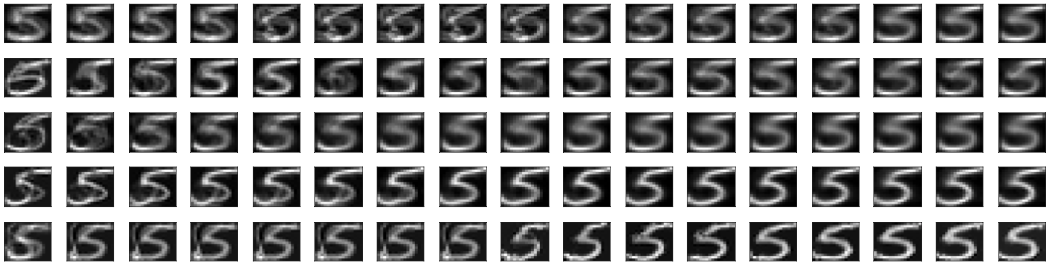
\includegraphics[width=\textwidth]{pic_paper/deformable3}\vspace{-.2cm}
%\caption{(USPS Digits) Estimation of the template. From top to bottom: batch, online, \ISAEM,\ \SAEMVR\ and \FISAEM\ through 7 epochs. Note that Batch method templates are replicated in-between epochs for a fair comparison with incremental variants. }\vspace{-.2cm}
%\label{fig:results}
%\end{center}
%\end{figure}
%\vspace{-0.2in}
%As the iterations proceed, the templates become sharper.
%Figure~\ref{fig:results} displays the virtue of the \SAEMVR\ and \FISAEM\ methods that obtain a more \textit{contrasted} and \textit{accurate} template estimate. 
%The incremental and online versions are better in the very first epochs compared to the batch method, given the high computational cost of the latter. 
%After a few epochs, the batch SAEM estimates similar template as the incremental and online methods due to their high variance. 
%Our variance reduced and fast incremental variants are effective in the long run and sharpen the template estimates contrasting between the background and the regions of interest in the image.
%
%\subsection{Pharmacokinetics (PK) Model with Absorption Lag Time}
%This numerical example was conducted in order to characterize the pharmacokinetics (PK) of orally administered drug to simulated patients, using a population pharmacokinetics approach. $M = 50$ synthetic datasets were generated for $n = 5000$ patients with $10$ observations (concentration measures) per patient.
%The goal is to model the evolution of the concentration of the absorbed drug using a \emph{nonlinear} and \emph{latent} variable model. 
%
%\vspace{0.08in}
%\noindent \textbf{Model and Explicit Updates:}
%We consider a one-compartment PK model for oral administration with an absorption lag-time ($T^{\textrm{lag}}$), assuming first-order absorption and linear elimination processes.
%The final model includes the following variables: $ka$ the absorption rate constant, $V$ the volume of distribution, $k$ the elimination rate constant and $T^{\textrm{lag}}$ the absorption lag-time. 
%We also add several covariates to our model such as $D$ the dose of drug administered, $t$ the time at which measures are taken and the weight of the patient influencing the volume $V$. More precisely, the log-volume $\log(V)$ is a linear function of the log-weight $lw70= \log(wt/70)$.
%Let $ z_i=(T_i^{\textrm{lag}}, ka_i, V_i, k_i)$ be the vector of individual PK parameters, different for each individual $i$.
%The final model reads:
%\begin{equation} \label{eq:pkmodel}
%y_{ij} = f(t_{ij},z_i)+ \varepsilon_{ij} \quad \textrm{where} \quad f(t_{ij},z_i) = \frac{D\,ka_i}{V(ka_i - k_i)}(\exponential^{-ka_i\,(t_{ij} - T_i^{\textrm{lag}})}-\exponential^{-k_i\,(t_{ij} - T_i^{\textrm{lag}})})\eqs,
%\end{equation}
%where $y_{ij}$ is the $j$-th concentration measurement of the drug of dosage $D$ injected at time $t_{ij}$ for patient $i$.
%We assume in this example that the residual errors $\varepsilon_{ij}$ are independent and normally distributed with mean 0 and variance $\sigma^2$.
%Lognormal distributions are used for the four PK parameters:
%\begin{align}
%& \log(T_i^{\textrm{lag}}) \sim \mathcal{N}(\log(T^{\textrm{lag}}_{\rm pop}), \omega^2_{T^{\textrm{lag}}} ) \eqs, \log(ka_i) \sim \mathcal{N}(\log(ka_{\rm pop}), \omega^2_{ka})\eqs,\notag\\
%&\log(V_i) \sim \mathcal{N}(\log(V_{\rm pop}), \omega^2_{V})\eqs,
% \log(k_i) \sim \mathcal{N}(\log(k_{\rm pop}), \omega^2_{k})\eqs.\notag
%\end{align}
%We note that the complete model $(y,z)$ defined by \eqref{eq:pkmodel} belongs to the curved exponential family, which vector of sufficient statistics $S = \big(S_1(z),S_2(z),S_3(z) \big)$ reads:
%\beq \label{eq:suffstat_deformable3}
%\begin{split}
%S_1(z)  = \frac{1}{n} \sum_{i=1}^n z_i  ,  \quad S_2(z) =\frac{1}{n} \sum_{i=1}^n z_i^\top z_i  , \quad S_3(z)  = \frac{1}{n}  \sum_{i=1}^n  \left(y_i - f(t_{i},z_i)\right)^2
%\end{split}
%\eeq
%where we have noted $y_i$ and $t_i$ the vector of observations and time for each patient $i \in \inter$.
%At iteration $k$, and setting the number of MC samples to $1$ for the sake of clarity, the MC sampling $z_i^{(k)} \sim p(z_i |y_i, \theta^{(k)})$ is performed using a Metropolis-Hastings procedure detailed in Appendix~\ref{app:experiments}. The quantities $\stt^{(k+1)}$ and $\hat{\bss}^{(k+1)}$ are then updated according to the different methods introduced in our paper, see Table~\ref{alg:prox}.
%Finally the maximization step yields:
%$$ \overline{\param} ( {\bm s} )
%= \left( \hat{\bss}^{(k+1)}_1 , \hat{\bss}^{(k+1)}_2 - \hat{\bss}^{(k+1)}_1 \left(\hat{\bss}^{(k+1)}_1 \right)^\top ,\hat{\bss}^{(k+1)}_3\right)
%= \left(\overline{\bm{z_{\rm pop}}} ( \hat{\bss}^{(k+1)}), \overline{\bm{\omega_{z}}} ( \hat{\bss}^{(k+1)}), \overline{\bm{\sigma}} ( \hat{\bss}^{(k+1)})\right)$$
%%\beq \label{eq:mstep_pk}
%%\overline{\param} ( {\bm s} )
%%= \left(
%%\begin{array}{c}
%%\hat{\bss}^{(k+1)}_1 \\
%%\hat{\bss}^{(k+1)}_2 - \hat{\bss}^{(k+1)}_1 \left(\hat{\bss}^{(k+1)}_1 \right)^\top \vspace{.2cm} \\
%%\hat{\bss}^{(k+1)}_3
%%\end{array}
%%\right)
%%= \left(
%%\begin{array}{c}
%%\overline{\bm{z_{\rm pop}}} ( \hat{\bss}^{(k+1)}) \\
%%\overline{\bm{\omega_{z}}} ( \hat{\bss}^{(k+1)}) \\
%%\overline{\bm{\sigma}} ( \hat{\bss}^{(k+1)})
%%\end{array}
%%\right) \eqsp.
%%\eeq
%where $z_{\rm pop}$ denotes the vector of fixed effects $(T^{\textrm{lag}}_{\rm pop}, ka_{\rm pop}, V_{\rm pop}, k_{\rm pop})$.
%
%        
%\begin{wrapfigure}[13]{r}{3.9in}\vspace{-0.3in}
%\begin{center}
%%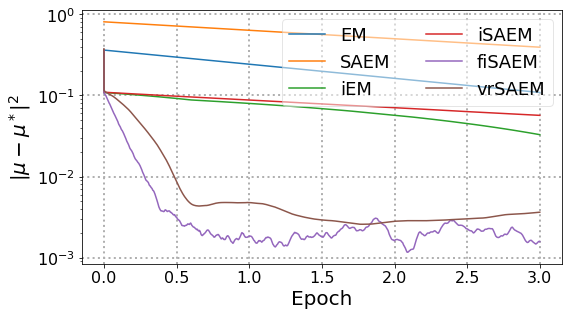
\includegraphics[width=2.5in]{pic_paper/tts_gmm_n100k.png}
%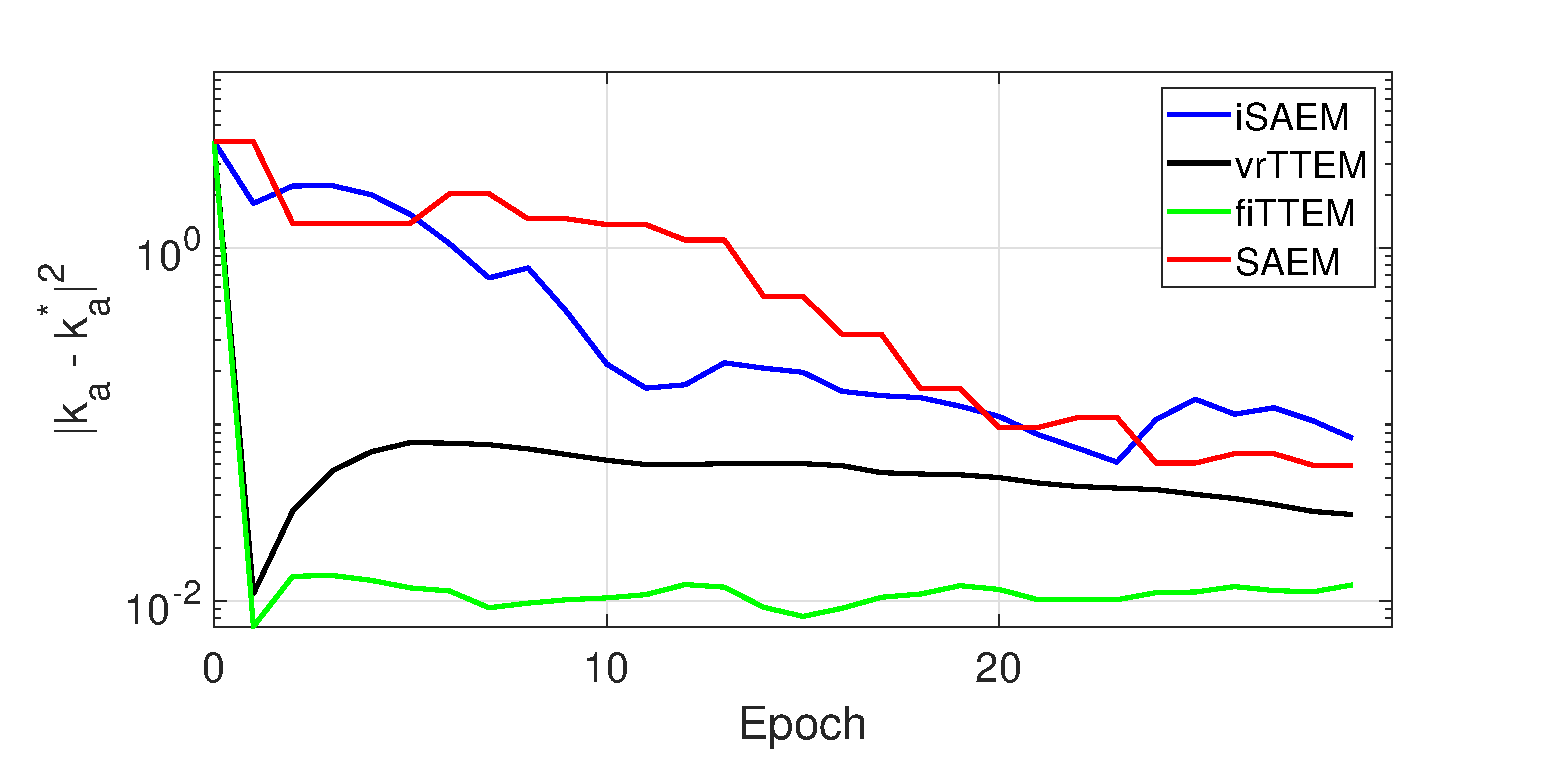
\includegraphics[width=3.9in]{fig/figpk.eps}\vspace{-.2cm}
%\end{center}
%\vspace{-0.1in}
%\caption{Precision $|ka^{(k)} - ka^*|^2$ per epoch}\vspace{-.2cm}
%\label{fig:pk_tts}
%\end{wrapfigure}
%
%\vspace{0.08in}
%\noindent \textbf{Monte Carlo study:}
%We conduct a Monte Carlo study to showcase the benefits of our scheme.
%$M=50$ datasets have been simulated using the following PK parameters values:
%$T^{\textrm{lag}}_{\rm pop} =1$, $ka_{\rm pop} =1$, $V_{\rm pop}= 8$, $k_{\rm pop}=0.1$, $ \omega_{T^{\textrm{lag}}}=0.4$, $\omega_{ka}=0.5$, $\omega_{V}=0.2$, $\omega_{k}=0.3$ and $\sigma^2=0.5$.
%We define the mean square distance over the $M$ replicates $E_k(\ell) = \frac{1}{M}\sum_{m=1}^{M}{\left(\theta_k^{(m)}(\ell) - \theta^* \right)^2}$ and plot it against the epochs (passes over the data) in Figure~\ref{fig:pk_tts}.	
%Note that the {\sf MC-step} \eqref{eq:mcstep} is performed using a Metropolis Hastings procedure since the posterior distribution under the model $\theta$ noted $p(z_i | y_i, \theta)$ is intractable, mainly due to the nonlinearity of the model \eqref{eq:pkmodel}.
%Figure~\ref{fig:pk_tts} shows clear advantage of variance reduced methods (\SAEMVR\ and \FISAEM\ ) avoiding the twists and turns displayed by the incremental and the batch methods (iSAEM and SAEM).





\section{Conclusion}


This paper introduces a new class of two-timescale EM methods for learning latent variable models.
In particular, the models dealt with in this paper belong to the curved exponential family and are possibly nonconvex.
The nonconvexity of the problem is tackled using a Robbins-Monro type of update, which represents the \textit{first level} of our class of methods.
The scalability with the number of samples is performed through a variance reduced and incremental update, the \textit{second} and last level of our newly introduced scheme.
The various algorithms are interpreted as scaled gradient methods, in the space of the sufficient statistics, and our convergence results are \emph{global}, in the sense of independence of the initial values, and \emph{non-asymptotic}, \ie true for any random termination number.
Numerical examples illustrate the benefits of our scheme on synthetic and real tasks.

%%%%%%
%% Appendix:
%% If needed a single appendix is created by
%%
%\appendix
%%
%% If several appendices are needed, then the command
%%
% \appendices
%%
%% in combination with further \section-commands can be used.
%%%%%%


\section*{Acknowledgment}

We are indebted to Michael Shell for maintaining and improving
\texttt{IEEEtran.cls}. 


%%%%%%
%% To balance the columns at the last page of the paper use this
%% command:
%%
%\enlargethispage{-1.2cm} 
%%
%% If the balancing should occur in the middle of the references, use
%% the following trigger:
%%
%\IEEEtriggeratref{3}
%%
%% which triggers a \newpage (i.e., new column) just before the given
%% reference number. Note that you need to adapt this if you modify
%% the paper.  The "triggered" command can be changed if desired:
%%
%\IEEEtriggercmd{\enlargethispage{-20cm}}
%%
%%%%%%


%%%%%%
%% References:
%% We recommend the usage of BibTeX:
%%
\bibliographystyle{IEEEtran}
\bibliography{references}
%%
%% where we here have assume the existence of the files
%% definitions.bib and bibliofile.bib.
%% BibTeX documentation can be obtained at:
%% http://www.ctan.org/tex-archive/biblio/bibtex/contrib/doc/
%%%%%%


%% Or you use manual references (pay attention to consistency and the
%% formatting style!):
%\begin{thebibliography}{9}
%
%\bibitem{Laport:LaTeX}
%L.~Lamport,
%  \emph{\LaTeX: A Document Preparation System,} 
%  Addison-Wesley, Reading, Massachusetts, USA, 2nd~ed., 1994. 
%
%\bibitem{GMS:LaTeXComp}
%F.~Mittelbach, M,~Goossens, J.~Braams, D.~Carlisle, and
%C.~Rowley, \emph{The {\LaTeX} Companion,} Addison-Wesley,
%Reading, Massachusetts, USA, 2nd~ed., 2004.
%
%\bibitem{oetiker_latex}
%T.~Oetiker, H.~Partl, I.~Hyna, and E.~Schlegl, \emph{The Not So Short
%  Introduction to {\LaTeX2e}}, version 5.06, Jun.~20, 2016. [Online].
%  Available: \url{https://tobi.oetiker.ch/lshort/}
%
%\bibitem{typesetmoser}
%S.~M. Moser, \emph{How to Typeset Equations in {\LaTeX}}, version 4.6,
%  Sep. 29, 2017. [Online]. Available:
%  \url{http://moser-isi.ethz.ch/manuals.html#eqlatex}
%
%\bibitem{IEEE:pdfsettings}
%IEEE, \emph{Preparing Conference Content for the IEEE Xplore Digital
%  Library.} [Online]. Available:
%  \url{http://www.ieee.org/conferences_events/conferences/organizers/pubs/preparing_content.html}
%
%\bibitem{IEEE:AuthorToolbox}
%IEEE, \emph{Author Digital Toolbox.} [Online.] Available:
%  \url{http://www.ieee.org/publications_standards/publications/authors/authors_journals.html}
%
%\end{thebibliography}


\end{document}


%%%%%%
%% Some comments about useful packages
%% (extract from bare_conf.tex by Michael Shell)
%%

% *** MISC UTILITY PACKAGES ***
%
%\usepackage{ifpdf}
% Heiko Oberdiek's ifpdf.sty is very useful if you need conditional
% compilation based on whether the output is pdf or dvi.
% usage:
% \ifpdf
%   % pdf code
% \else
%   % dvi code
% \fi
% The latest version of ifpdf.sty can be obtained from:
% http://www.ctan.org/pkg/ifpdf
% Also, note that IEEEtran.cls V1.7 and later provides a builtin
% \ifCLASSINFOpdf conditional that works the same way.
% When switching from latex to pdflatex and vice-versa, the compiler may
% have to be run twice to clear warning/error messages.


% *** CITATION PACKAGES ***
%
%\usepackage{cite}
% cite.sty was written by Donald Arseneau
% V1.6 and later of IEEEtran pre-defines the format of the cite.sty package
% \cite{} output to follow that of the IEEE. Loading the cite package will
% result in citation numbers being automatically sorted and properly
% "compressed/ranged". e.g., [1], [9], [2], [7], [5], [6] without using
% cite.sty will become [1], [2], [5]--[7], [9] using cite.sty. cite.sty's
% \cite will automatically add leading space, if needed. Use cite.sty's
% noadjust option (cite.sty V3.8 and later) if you want to turn this off
% such as if a citation ever needs to be enclosed in parenthesis.
% cite.sty is already installed on most LaTeX systems. Be sure and use
% version 5.0 (2009-03-20) and later if using hyperref.sty.
% The latest version can be obtained at:
% http://www.ctan.org/pkg/cite
% The documentation is contained in the cite.sty file itself.


% *** GRAPHICS RELATED PACKAGES ***
%
\ifCLASSINFOpdf
  % \usepackage[pdftex]{graphicx}
  % declare the path(s) where your graphic files are
  % \graphicspath{{../pdf/}{../jpeg/}}
  % and their extensions so you won't have to specify these with
  % every instance of \includegraphics
  % \DeclareGraphicsExtensions{.pdf,.jpeg,.png}
\else
  % or other class option (dvipsone, dvipdf, if not using dvips). graphicx
  % will default to the driver specified in the system graphics.cfg if no
  % driver is specified.
  % \usepackage[dvips]{graphicx}
  % declare the path(s) where your graphic files are
  % \graphicspath{{../eps/}}
  % and their extensions so you won't have to specify these with
  % every instance of \includegraphics
  % \DeclareGraphicsExtensions{.eps}
\fi
% graphicx was written by David Carlisle and Sebastian Rahtz. It is
% required if you want graphics, photos, etc. graphicx.sty is already
% installed on most LaTeX systems. The latest version and documentation
% can be obtained at: 
% http://www.ctan.org/pkg/graphicx
% Another good source of documentation is "Using Imported Graphics in
% LaTeX2e" by Keith Reckdahl which can be found at:
% http://www.ctan.org/pkg/epslatex
%
% latex, and pdflatex in dvi mode, support graphics in encapsulated
% postscript (.eps) format. pdflatex in pdf mode supports graphics
% in .pdf, .jpeg, .png and .mps (metapost) formats. Users should ensure
% that all non-photo figures use a vector format (.eps, .pdf, .mps) and
% not a bitmapped formats (.jpeg, .png). The IEEE frowns on bitmapped formats
% which can result in "jaggedy"/blurry rendering of lines and letters as
% well as large increases in file sizes.
%
% You can find documentation about the pdfTeX application at:
% http://www.tug.org/applications/pdftex


% *** MATH PACKAGES ***
%
%\usepackage{amsmath}
% A popular package from the American Mathematical Society that provides
% many useful and powerful commands for dealing with mathematics.
%
% Note that the amsmath package sets \interdisplaylinepenalty to 10000
% thus preventing page breaks from occurring within multiline equations. Use:
%\interdisplaylinepenalty=2500
% after loading amsmath to restore such page breaks as IEEEtran.cls normally
% does. amsmath.sty is already installed on most LaTeX systems. The latest
% version and documentation can be obtained at:
% http://www.ctan.org/pkg/amsmath


% *** SPECIALIZED LIST PACKAGES ***
%
%\usepackage{algorithmic}
% algorithmic.sty was written by Peter Williams and Rogerio Brito.
% This package provides an algorithmic environment fo describing algorithms.
% You can use the algorithmic environment in-text or within a figure
% environment to provide for a floating algorithm. Do NOT use the algorithm
% floating environment provided by algorithm.sty (by the same authors) or
% algorithm2e.sty (by Christophe Fiorio) as the IEEE does not use dedicated
% algorithm float types and packages that provide these will not provide
% correct IEEE style captions. The latest version and documentation of
% algorithmic.sty can be obtained at:
% http://www.ctan.org/pkg/algorithms
% Also of interest may be the (relatively newer and more customizable)
% algorithmicx.sty package by Szasz Janos:
% http://www.ctan.org/pkg/algorithmicx


% *** ALIGNMENT PACKAGES ***
%
%\usepackage{array}
% Frank Mittelbach's and David Carlisle's array.sty patches and improves
% the standard LaTeX2e array and tabular environments to provide better
% appearance and additional user controls. As the default LaTeX2e table
% generation code is lacking to the point of almost being broken with
% respect to the quality of the end results, all users are strongly
% advised to use an enhanced (at the very least that provided by array.sty)
% set of table tools. array.sty is already installed on most systems. The
% latest version and documentation can be obtained at:
% http://www.ctan.org/pkg/array

% IEEEtran contains the IEEEeqnarray family of commands that can be used to
% generate multiline equations as well as matrices, tables, etc., of high
% quality.


% *** SUBFIGURE PACKAGES ***
%\ifCLASSOPTIONcompsoc
%  \usepackage[caption=false,font=normalsize,labelfont=sf,textfont=sf]{subfig}
%\else
%  \usepackage[caption=false,font=footnotesize]{subfig}
%\fi
% subfig.sty, written by Steven Douglas Cochran, is the modern replacement
% for subfigure.sty, the latter of which is no longer maintained and is
% incompatible with some LaTeX packages including fixltx2e. However,
% subfig.sty requires and automatically loads Axel Sommerfeldt's caption.sty
% which will override IEEEtran.cls' handling of captions and this will result
% in non-IEEE style figure/table captions. To prevent this problem, be sure
% and invoke subfig.sty's "caption=false" package option (available since
% subfig.sty version 1.3, 2005/06/28) as this is will preserve IEEEtran.cls
% handling of captions.
% Note that the Computer Society format requires a larger sans serif font
% than the serif footnote size font used in traditional IEEE formatting
% and thus the need to invoke different subfig.sty package options depending
% on whether compsoc mode has been enabled.
%
% The latest version and documentation of subfig.sty can be obtained at:
% http://www.ctan.org/pkg/subfig


% *** FLOAT PACKAGES ***
%
%\usepackage{fixltx2e}
% fixltx2e, the successor to the earlier fix2col.sty, was written by
% Frank Mittelbach and David Carlisle. This package corrects a few problems
% in the LaTeX2e kernel, the most notable of which is that in current
% LaTeX2e releases, the ordering of single and double column floats is not
% guaranteed to be preserved. Thus, an unpatched LaTeX2e can allow a
% single column figure to be placed prior to an earlier double column
% figure.
% Be aware that LaTeX2e kernels dated 2015 and later have fixltx2e.sty's
% corrections already built into the system in which case a warning will
% be issued if an attempt is made to load fixltx2e.sty as it is no longer
% needed.
% The latest version and documentation can be found at:
% http://www.ctan.org/pkg/fixltx2e


%\usepackage{stfloats}
% stfloats.sty was written by Sigitas Tolusis. This package gives LaTeX2e
% the ability to do double column floats at the bottom of the page as well
% as the top. (e.g., "\begin{figure*}[!b]" is not normally possible in
% LaTeX2e). It also provides a command:
%\fnbelowfloat
% to enable the placement of footnotes below bottom floats (the standard
% LaTeX2e kernel puts them above bottom floats). This is an invasive package
% which rewrites many portions of the LaTeX2e float routines. It may not work
% with other packages that modify the LaTeX2e float routines. The latest
% version and documentation can be obtained at:
% http://www.ctan.org/pkg/stfloats
% Do not use the stfloats baselinefloat ability as the IEEE does not allow
% \baselineskip to stretch. Authors submitting work to the IEEE should note
% that the IEEE rarely uses double column equations and that authors should try
% to avoid such use. Do not be tempted to use the cuted.sty or midfloat.sty
% packages (also by Sigitas Tolusis) as the IEEE does not format its papers in
% such ways.
% Do not attempt to use stfloats with fixltx2e as they are incompatible.
% Instead, use Morten Hogholm'a dblfloatfix which combines the features
% of both fixltx2e and stfloats:
%
% \usepackage{dblfloatfix}
% The latest version can be found at:
% http://www.ctan.org/pkg/dblfloatfix


% *** PDF and URL PACKAGES ***
%
%\usepackage{url}
% url.sty was written by Donald Arseneau. It provides better support for
% handling and breaking URLs. url.sty is already installed on most LaTeX
% systems. The latest version and documentation can be obtained at:
% http://www.ctan.org/pkg/url
% Basically, \url{my_url_here}.



% *** Do not adjust lengths that control margins, column widths, etc. ***
% *** Do not use packages that alter fonts (such as pslatex).         ***
%%%%%%


%%% Local Variables:
%%% mode: latex
%%% TeX-master: t
%%% End:
